\documentclass[12pt, a4paper, openany, twoside]{book}
\usepackage[italian]{babel}
\usepackage[T1]{fontenc}
\usepackage[utf8]{inputenc}
\usepackage{amsmath} 
\usepackage{xcolor}
\usepackage[margin=1in]{geometry}
\usepackage{hyperref}
\usepackage{graphicx}
\graphicspath{{./img/}}
\usepackage{tikz}
\hypersetup{
    colorlinks=true,
    linkcolor=blue,
    filecolor=magenta,      
    urlcolor=cyan,
}
%usepackage[latin1]{inputenc}
\begin{document}
\fontfamily{cmss}\selectfont
\pagestyle{plain}
\author{DaveRhapsody}
\title {Sistemi Distribuiti}
\date {11 Marzo 2020}
\maketitle
\tableofcontents
\chapter{Introduzione}
Un sistema distribuito è un insieme di componenti hardware e software che 
comunicano tramite scambi di messaggi in rete.
Il concetto di componente è fondamentale, può essere per l'appunto sia hardware
che software.
\paragraph{Nel dettaglio:} E' un sistema di componenti \textbf{autonome},
nel senso che le componenti sono indipendenti tra loro MA concorrono tutte
allo stesso scopo. Per apparire come unico componente occorre generare una
sorta di collaborazione \textbf{SENZA} memoria condivisa.
\paragraph{Autonomia:} Ognuno svolge il proprio compito in modo indipendente
(sia in termini di tempo che dati) da ogni altro. Pertanto occorre che le
componenti siano \textbf{SINCRONIZZATE} (Reti e Sistemi insegna ->).
Questo insieme di nodi appaiono all'utente finale come un unico sistema
\textbf{coerente} senza che lui sappia dove vengono processati (e nemmeno
come) i dati. Il sistema è un blocco unico agli occhi dell'utente MA obv no.
\paragraph{Concetto di trasparenza:} Il livello di trasparenza lo si decide 
in fase di progettazione del sistema, fondamentalmente è il livello tale per 
cui l'utente sappia come vengono processati i dati, e cosa e come viene
eseguito dal sistema. (Un sistema trasparente, è un sistema che ti fa
vedere vita, morte, miracoli, luci, coriandoli, sassi e Babbo Natale).
\section{Caratteristiche fondamentali}
\begin{itemize}
	\item Non c'è memoria condivisa
	\item L'esecuzione è concorrente (allo stesso istante)
	\item Non ci sono stati del processo o della memoria, ogni nodo è a sè un
	processo!
	\item NON C'E' UN CLOCK GLOBALE, niente scheduling. controllo (globale),
	si fa tutto per scambio di messaggi
	\item Non esiste un fallimento globale ma un fallimento della singola
	componente. 
	\paragraph{Sistemi Realtime:} Noi non utilizziamo questo genere di 
	dispositivi, studiamo e prendiamo in esame dispositivi best-effort
	\item Architetture software
\end{itemize}
\section{Architetture software}
E' la struttura del sistema, di come sono organizzate le componenti, quali
sono i protocolli, le interfacce, etc.
\begin{itemize}
	\item Architetture a Livelli (tier)
	\item Architetture a oggetti
	\item Architetture centrate sui dati
	\item Architetture event-based (ajax)
\end{itemize}
\subsection{Stratificazione}
L'idea è formare degli strati di complessità, fondamentalmente nulla vieta di 
fare tutto a livello application, lì si impreca per davvero, ma soprattutto
non ci sarebbe una specializzazione. Il motto è "Fai una cosa, ma falla bene".
\section{Tipi di sistemi operativi}
In base al tipo ho un livello diverso di trasparenza
\begin{itemize}
	\item DOS: Distributed OS
	\item NOS: Network OS: L'OS ti dà delle librerie e supporti per supportare
	delle applicazioni MA non nasconde le comunicazioni tra le varie applicazioni.
	\item Middleware: Hai un insieme di sistemi di rete che forniscono primitive
	per sostenere comunicazione tra sistemi E costruirci delle logiche che 
	consentano di vedere questo come unico sistema (Sì, il middleware è 
	a sua volta un'applicazione distribuita)
	\section{Servizi del middleware}
	\begin{itemize}
		\item Naming
		\item Accesso trasparente
		\item Persisenza: avviene una memorizzazione di dati persistente
		\item Transazioni distribuite: Va garantita la consistenza dei dati
		\item Sicurezza dei dati: integrità computazionali
	\end{itemize}
	\paragraph{Riporto il riassunto presente nelle slides}  
	\begin{center}
	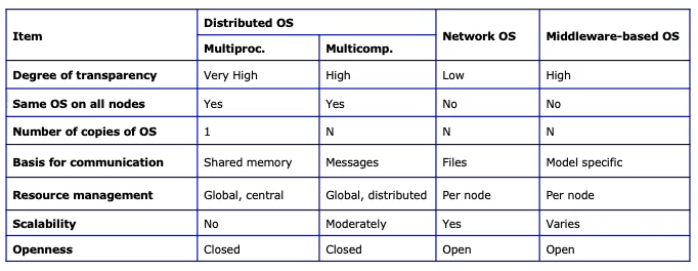
\includegraphics[width=0.75\textwidth]{1.png}
	\end{center}
\end{itemize}
\chapter{Modello Client-Server}
E' un'interazione basata su richiesta-risposta tra una componente e 
l'altra.
\paragraph{Funzionamento:}
\begin{enumerate}
	\item Client invia la request
	\item Server la riceve, client aspetta
	\item Server elabora
	\item Server risponde alla richiesta
\end{enumerate}
Quando client aspetta, quest'ultimo è in standby, in attesa, fermo, inchiodato.
Il server si attiva ad ogni richiesta che arriva. Richiesta e risposta hanno
un tempo ovviamente proprio, che deriva dalla rete di riferimento, chiaramente
se si fa tutto sulla stessa macchina si parla di microsecondi.
\paragraph{Osservazione:} Un dispositivo è sia client che server, può essere
sia uno che l'altro.
\paragraph{Tipi di accesso:}
\begin{itemize}
	\item Accesso a server multipli (nel senso che sono duplicati i server)
	\item Accesso via proxy
\end{itemize}
\section{Problemi dei Sistemi Distribuiti}
\begin{itemize}
	\item Identificazione della controparte: Identifico la risorsa, tipo con
	address etc.
	\item Accesso alla controparte: Dove accedo? Chi è il mio access point
	\item Comunicazione 1: Definisco il formato dei messaggi scambiati
	\item Comunicazione 2: Capisco il contenuto del messaggio in seguito 
	all'estrazione
	\paragraph{Esempio:} I tipi per i dati, che specificano un insieme 
	di valori ed operazioni fattibili su un determinato dato.
\end{itemize}
\section{Trasparenza}
Significa nascondere all'utente \textbf{come} viene ottenuto un determinato
risultato. E' per intenderci ciò che salva coloro che programmano tutto nel 
main.
Come si fa?
\begin{itemize}
	\item \textbf{Naming}: non mi connetto per indirizzo IP ma per indirizzo web, link.
	\item \textbf{Accesso trasparente}: Come accedo in maniera trasparente? Anche qui
	nomi simbolici, qualcosa che non mi faccia capire la locazione della 
	controparte
	\item \textbf{Location Trasparency}: Hai una stampante a casa e devi stampare una foto
	di gattini? Ti serve sapere dove si trova, non puoi cercare a caso su google,
	quindi devi sapere fisicamente dove hai la stampante. Invece se ti serve
	una calcolatrice online tipo wolfram alpha, digiti l'equazione, la risolve,
	ma tu non sai una bega di dove è stata risolta.
	\item \textbf{Relocation o trasparenza mobile}: Posso spostare le risorse mentre le
	uso (Cellulari, dispositivi wifi, ci siamo capiti).
	\item \textbf{Migrazione}: Posso spostare un sito web da un pc del 91 ad un pc del 
	2020, il servizio quello è, cambierà la velocità (tempi di elaborazione
	+ request + response)
	\item \textbf{Replicazione}: Hai una serie di server identici, tu ti connetti ad uno
	o l'altro, cambia niente
	\item \textbf{Concorrenza}: In più utenti accediamo allo stesso servizio (spotify)
	\item \textbf{Trasparenza del fallimento}: Ciò che resta dopo un fallimento di una
	componente deve colmare i danni di una componente morta.
	\item \textbf{Persistenza}: Non mi accorgo di quando un sistema è riavviato o no
\end{itemize}
In alcuni casi è impossibile nascondere un fail o lo stato di una applicazione,
se ti crasha Word, vedi che ti è crashato Word, quindi in qualche modo 
va comunicato all'utente "Ueh, fa schifo Uord, usa OpeNoFFiSsszsxxs". Ma
tra l'altro non sempre è utile nascondere, prendete l'esempio di prima della
stampante. 
\section{Separazione tra interfaccia e realizzazione}
Costruisco un'astrazione logica che nasconde i dettagli implementativi
di ciò che sta diestro. Ogni componente pubblica il What cioè COSA fa, ma non
ti spara fuori anche l'HOW, cioè COME lo fa, è il concetto di information
hiding di Java.
\paragraph{Esempio:}
Gestione delle stringhe nei vari linguaggi. Una stringa è una concatenazione
di caratteri, la gestione di append, copy, concat etc. sono how, il 
risultato finale è il what
\section{Politiche versus mechanism}
Un Sistema distribuito è composto da.. Va beh avete capito. Progressivamente
si va verso un unico enorme (utopico) sistema complesso organizzato con delle
policy stabilite. 
Le politiche banalmente sono una serie di regole ad esempio prendete il context
switch di Unix. 
\begin{itemize}
	\item Il CS è un meccanismo
	\item Il Round Robin invece è la policy di come è gestito un comportamento	
\end{itemize}
\section{Concetto di protocollo}
Un protocollo è un insieme di regole che definiscono un formato, l'ordine,
payload, operazioni da compiere alla ricezione od all'invio di un 
messaggio.


    
















\end{document}